\documentclass[1p]{elsarticle_modified}
%\bibliographystyle{elsarticle-num}

%\usepackage[colorlinks]{hyperref}
%\usepackage{abbrmath_seonhwa} %\Abb, \Ascr, \Acal ,\Abf, \Afrak
\usepackage{amsfonts}
\usepackage{amssymb}
\usepackage{amsmath}
\usepackage{amsthm}
\usepackage{scalefnt}
\usepackage{amsbsy}
\usepackage{kotex}
\usepackage{caption}
\usepackage{subfig}
\usepackage{color}
\usepackage{graphicx}
\usepackage{xcolor} %% white, black, red, green, blue, cyan, magenta, yellow
\usepackage{float}
\usepackage{setspace}
\usepackage{hyperref}

\usepackage{tikz}
\usetikzlibrary{arrows}

\usepackage{multirow}
\usepackage{array} % fixed length table
\usepackage{hhline}

%%%%%%%%%%%%%%%%%%%%%
\makeatletter
\renewcommand*\env@matrix[1][\arraystretch]{%
	\edef\arraystretch{#1}%
	\hskip -\arraycolsep
	\let\@ifnextchar\new@ifnextchar
	\array{*\c@MaxMatrixCols c}}
\makeatother %https://tex.stackexchange.com/questions/14071/how-can-i-increase-the-line-spacing-in-a-matrix
%%%%%%%%%%%%%%%

\usepackage[normalem]{ulem}

\newcommand{\msout}[1]{\ifmmode\text{\sout{\ensuremath{#1}}}\else\sout{#1}\fi}
%SOURCE: \msout is \stkout macro in https://tex.stackexchange.com/questions/20609/strikeout-in-math-mode

\newcommand{\cancel}[1]{
	\ifmmode
	{\color{red}\msout{#1}}
	\else
	{\color{red}\sout{#1}}
	\fi
}

\newcommand{\add}[1]{
	{\color{blue}\uwave{#1}}
}

\newcommand{\replace}[2]{
	\ifmmode
	{\color{red}\msout{#1}}{\color{blue}\uwave{#2}}
	\else
	{\color{red}\sout{#1}}{\color{blue}\uwave{#2}}
	\fi
}

\newcommand{\Sol}{\mathcal{S}} %segment
\newcommand{\D}{D} %diagram
\newcommand{\A}{\mathcal{A}} %arc


%%%%%%%%%%%%%%%%%%%%%%%%%%%%%5 test

\def\sl{\operatorname{\textup{SL}}(2,\Cbb)}
\def\psl{\operatorname{\textup{PSL}}(2,\Cbb)}
\def\quan{\mkern 1mu \triangleright \mkern 1mu}

\theoremstyle{definition}
\newtheorem{thm}{Theorem}[section]
\newtheorem{prop}[thm]{Proposition}
\newtheorem{lem}[thm]{Lemma}
\newtheorem{ques}[thm]{Question}
\newtheorem{cor}[thm]{Corollary}
\newtheorem{defn}[thm]{Definition}
\newtheorem{exam}[thm]{Example}
\newtheorem{rmk}[thm]{Remark}
\newtheorem{alg}[thm]{Algorithm}

\newcommand{\I}{\sqrt{-1}}
\begin{document}

%\begin{frontmatter}
%
%\title{Boundary parabolic representations of knots up to 8 crossings}
%
%%% Group authors per affiliation:
%\author{Yunhi Cho} 
%\address{Department of Mathematics, University of Seoul, Seoul, Korea}
%\ead{yhcho@uos.ac.kr}
%
%
%\author{Seonhwa Kim} %\fnref{s_kim}}
%\address{Center for Geometry and Physics, Institute for Basic Science, Pohang, 37673, Korea}
%\ead{ryeona17@ibs.re.kr}
%
%\author{Hyuk Kim}
%\address{Department of Mathematical Sciences, Seoul National University, Seoul 08826, Korea}
%\ead{hyukkim@snu.ac.kr}
%
%\author{Seokbeom Yoon}
%\address{Department of Mathematical Sciences, Seoul National University, Seoul, 08826,  Korea}
%\ead{sbyoon15@snu.ac.kr}
%
%\begin{abstract}
%We find all boundary parabolic representation of knots up to 8 crossings.
%
%\end{abstract}
%\begin{keyword}
%    \MSC[2010] 57M25 
%\end{keyword}
%
%\end{frontmatter}

%\linenumbers
%\tableofcontents
%
\newcommand\colored[1]{\textcolor{white}{\rule[-0.35ex]{0.8em}{1.4ex}}\kern-0.8em\color{red} #1}%
%\newcommand\colored[1]{\textcolor{white}{ #1}\kern-2.17ex	\textcolor{white}{ #1}\kern-1.81ex	\textcolor{white}{ #1}\kern-2.15ex\color{red}#1	}

{\Large $\underline{12n_{0208}~(K12n_{0208})}$}

\setlength{\tabcolsep}{10pt}
\renewcommand{\arraystretch}{1.6}
\vspace{1cm}\begin{tabular}{m{100pt}>{\centering\arraybackslash}m{274pt}}
\multirow{5}{120pt}{
	\centering
	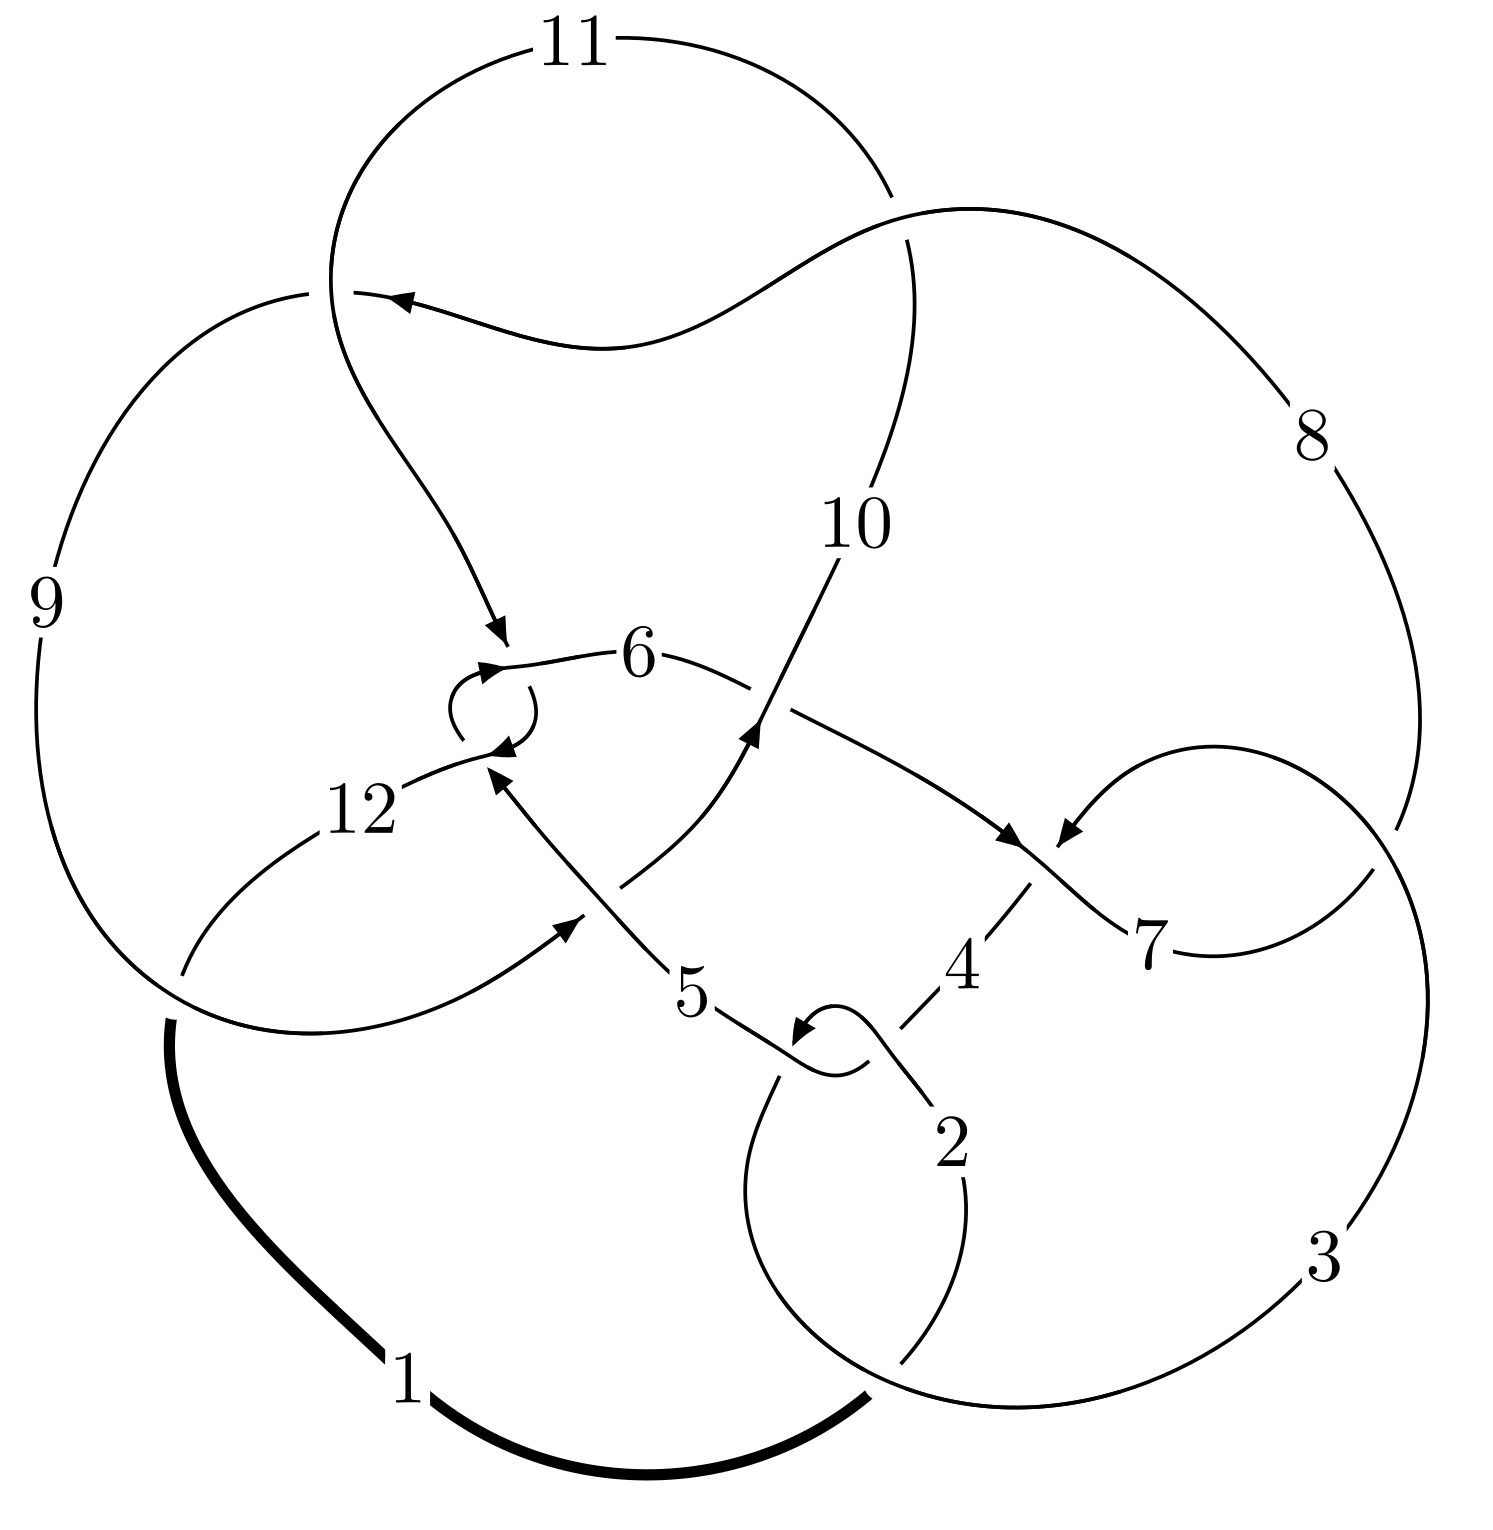
\includegraphics[width=112pt]{../../../GIT/diagram.site/Diagrams/png/2297_12n_0208.png}\\
\ \ \ A knot diagram\footnotemark}&
\allowdisplaybreaks
\textbf{Linearized knot diagam} \\
\cline{2-2}
 &
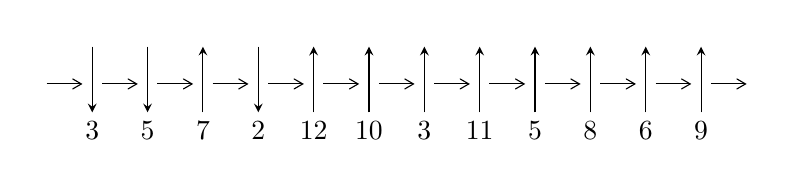
\begin{tikzpicture}[x=20pt, y=17pt]
	% nodes
	\node (C0) at (0, 0) {};
	\node (C1) at (1, 0) {};
	\node (C1U) at (1, +1) {};
	\node (C1D) at (1, -1) {3};

	\node (C2) at (2, 0) {};
	\node (C2U) at (2, +1) {};
	\node (C2D) at (2, -1) {5};

	\node (C3) at (3, 0) {};
	\node (C3U) at (3, +1) {};
	\node (C3D) at (3, -1) {7};

	\node (C4) at (4, 0) {};
	\node (C4U) at (4, +1) {};
	\node (C4D) at (4, -1) {2};

	\node (C5) at (5, 0) {};
	\node (C5U) at (5, +1) {};
	\node (C5D) at (5, -1) {12};

	\node (C6) at (6, 0) {};
	\node (C6U) at (6, +1) {};
	\node (C6D) at (6, -1) {10};

	\node (C7) at (7, 0) {};
	\node (C7U) at (7, +1) {};
	\node (C7D) at (7, -1) {3};

	\node (C8) at (8, 0) {};
	\node (C8U) at (8, +1) {};
	\node (C8D) at (8, -1) {11};

	\node (C9) at (9, 0) {};
	\node (C9U) at (9, +1) {};
	\node (C9D) at (9, -1) {5};

	\node (C10) at (10, 0) {};
	\node (C10U) at (10, +1) {};
	\node (C10D) at (10, -1) {8};

	\node (C11) at (11, 0) {};
	\node (C11U) at (11, +1) {};
	\node (C11D) at (11, -1) {6};

	\node (C12) at (12, 0) {};
	\node (C12U) at (12, +1) {};
	\node (C12D) at (12, -1) {9};
	\node (C13) at (13, 0) {};

	% arrows
	\draw[->,>={angle 60}]
	(C0) edge (C1) (C1) edge (C2) (C2) edge (C3) (C3) edge (C4) (C4) edge (C5) (C5) edge (C6) (C6) edge (C7) (C7) edge (C8) (C8) edge (C9) (C9) edge (C10) (C10) edge (C11) (C11) edge (C12) (C12) edge (C13) ;	\draw[->,>=stealth]
	(C1U) edge (C1D) (C2U) edge (C2D) (C3D) edge (C3U) (C4U) edge (C4D) (C5D) edge (C5U) (C6D) edge (C6U) (C7D) edge (C7U) (C8D) edge (C8U) (C9D) edge (C9U) (C10D) edge (C10U) (C11D) edge (C11U) (C12D) edge (C12U) ;
	\end{tikzpicture} \\
\hhline{~~} \\& 
\textbf{Solving Sequence} \\ \cline{2-2} 
 &
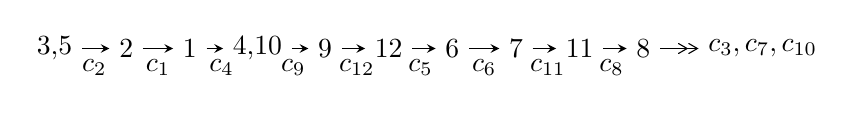
\begin{tikzpicture}[x=23pt, y=7pt]
	% node
	\node (A0) at (-1/8, 0) {3,5};
	\node (A1) at (1, 0) {2};
	\node (A2) at (2, 0) {1};
	\node (A3) at (49/16, 0) {4,10};
	\node (A4) at (33/8, 0) {9};
	\node (A5) at (41/8, 0) {12};
	\node (A6) at (49/8, 0) {6};
	\node (A7) at (57/8, 0) {7};
	\node (A8) at (65/8, 0) {11};
	\node (A9) at (73/8, 0) {8};
	\node (C1) at (1/2, -1) {$c_{2}$};
	\node (C2) at (3/2, -1) {$c_{1}$};
	\node (C3) at (5/2, -1) {$c_{4}$};
	\node (C4) at (29/8, -1) {$c_{9}$};
	\node (C5) at (37/8, -1) {$c_{12}$};
	\node (C6) at (45/8, -1) {$c_{5}$};
	\node (C7) at (53/8, -1) {$c_{6}$};
	\node (C8) at (61/8, -1) {$c_{11}$};
	\node (C9) at (69/8, -1) {$c_{8}$};
	\node (A10) at (11, 0) {$c_{3},c_{7},c_{10}$};

	% edge
	\draw[->,>=stealth]	
	(A0) edge (A1) (A1) edge (A2) (A2) edge (A3) (A3) edge (A4) (A4) edge (A5) (A5) edge (A6) (A6) edge (A7) (A7) edge (A8) (A8) edge (A9) ;
	\draw[->>,>={angle 60}]	
	(A9) edge (A10);
\end{tikzpicture} \\ 

\end{tabular} \\

\footnotetext{
The image of knot diagram is generated by the software ``\textbf{Draw programme}" developed by Andrew Bartholomew(\url{http://www.layer8.co.uk/maths/draw/index.htm\#Running-draw}), where we modified some parts for our purpose(\url{https://github.com/CATsTAILs/LinksPainter}).
}\phantom \\ \newline 
\centering \textbf{Ideals for irreducible components\footnotemark of $X_{\text{par}}$} 
 
\begin{align*}
I^u_{1}&=\langle 
6.08795\times10^{88} u^{64}+5.17375\times10^{89} u^{63}+\cdots+3.20686\times10^{88} b-2.93483\times10^{88},\\
\phantom{I^u_{1}}&\phantom{= \langle  }4.89867\times10^{87} u^{64}+3.97189\times10^{88} u^{63}+\cdots+3.56318\times10^{87} a+1.88337\times10^{88},\;u^{65}+10 u^{64}+\cdots-11 u-1\rangle \\
I^u_{2}&=\langle 
- a^6+2 a^4-3 a^2+b+2,\;a^8- a^7- a^6+2 a^5+a^4-2 a^3+2 a-1,\;u-1\rangle \\
I^u_{3}&=\langle 
- u^5-4 u^4-3 u^3+2 u^2+3 b+3 u+1,\;a,\;u^6+u^5- u^4-2 u^3+u+1\rangle \\
\\
\end{align*}
\raggedright * 3 irreducible components of $\dim_{\mathbb{C}}=0$, with total 79 representations.\\
\footnotetext{All coefficients of polynomials are rational numbers. But the coefficients are sometimes approximated in decimal forms when there is not enough margin.}
\newpage
\renewcommand{\arraystretch}{1}
\centering \section*{I. $I^u_{1}= \langle 6.09\times10^{88} u^{64}+5.17\times10^{89} u^{63}+\cdots+3.21\times10^{88} b-2.93\times10^{88},\;4.90\times10^{87} u^{64}+3.97\times10^{88} u^{63}+\cdots+3.56\times10^{87} a+1.88\times10^{88},\;u^{65}+10 u^{64}+\cdots-11 u-1 \rangle$}
\flushleft \textbf{(i) Arc colorings}\\
\begin{tabular}{m{7pt} m{180pt} m{7pt} m{180pt} }
\flushright $a_{3}=$&$\begin{pmatrix}1\\0\end{pmatrix}$ \\
\flushright $a_{5}=$&$\begin{pmatrix}0\\u\end{pmatrix}$ \\
\flushright $a_{2}=$&$\begin{pmatrix}1\\- u^2\end{pmatrix}$ \\
\flushright $a_{1}=$&$\begin{pmatrix}- u^2+1\\- u^2\end{pmatrix}$ \\
\flushright $a_{4}=$&$\begin{pmatrix}u\\- u^3+u\end{pmatrix}$ \\
\flushright $a_{10}=$&$\begin{pmatrix}-1.37480 u^{64}-11.1470 u^{63}+\cdots+1.59486 u-5.28564\\-1.89841 u^{64}-16.1334 u^{63}+\cdots+13.3331 u+0.915173\end{pmatrix}$ \\
\flushright $a_{9}=$&$\begin{pmatrix}-1.37480 u^{64}-11.1470 u^{63}+\cdots+1.59486 u-5.28564\\-5.70850 u^{64}-48.6155 u^{63}+\cdots+40.5692 u+3.51616\end{pmatrix}$ \\
\flushright $a_{12}=$&$\begin{pmatrix}-0.0863684 u^{64}-0.904473 u^{63}+\cdots-10.1953 u+2.73218\\4.03669 u^{64}+33.9170 u^{63}+\cdots-25.9308 u-2.40433\end{pmatrix}$ \\
\flushright $a_{6}=$&$\begin{pmatrix}2.43925 u^{64}+21.4354 u^{63}+\cdots-19.0226 u-2.35834\\-0.459002 u^{64}-3.41692 u^{63}+\cdots+0.298030 u-0.146156\end{pmatrix}$ \\
\flushright $a_{7}=$&$\begin{pmatrix}-3.90567 u^{64}-32.4081 u^{63}+\cdots+19.3485 u-1.64653\\3.74879 u^{64}+31.7029 u^{63}+\cdots-24.6208 u-2.74300\end{pmatrix}$ \\
\flushright $a_{11}=$&$\begin{pmatrix}0.156882 u^{64}+0.705201 u^{63}+\cdots+5.27226 u+4.38953\\6.31020 u^{64}+53.4331 u^{63}+\cdots-41.9173 u-3.84100\end{pmatrix}$ \\
\flushright $a_{8}=$&$\begin{pmatrix}-0.156882 u^{64}-0.705201 u^{63}+\cdots-5.27226 u-4.38953\\3.74879 u^{64}+31.7029 u^{63}+\cdots-24.6208 u-2.74300\end{pmatrix}$\\&\end{tabular}
\flushleft \textbf{(ii) Obstruction class $= -1$}\\~\\
\flushleft \textbf{(iii) Cusp Shapes $= 8.74709 u^{64}+73.9059 u^{63}+\cdots-57.9278 u+8.32578$}\\~\\
\newpage\renewcommand{\arraystretch}{1}
\flushleft \textbf{(iv) u-Polynomials at the component}\newline \\
\begin{tabular}{m{50pt}|m{274pt}}
Crossings & \hspace{64pt}u-Polynomials at each crossing \\
\hline $$\begin{aligned}c_{1}\end{aligned}$$&$\begin{aligned}
&u^{65}+68 u^{64}+\cdots+59 u+1
\end{aligned}$\\
\hline $$\begin{aligned}c_{2},c_{4}\end{aligned}$$&$\begin{aligned}
&u^{65}-10 u^{64}+\cdots-11 u+1
\end{aligned}$\\
\hline $$\begin{aligned}c_{3},c_{7}\end{aligned}$$&$\begin{aligned}
&u^{65}-2 u^{64}+\cdots+640 u-256
\end{aligned}$\\
\hline $$\begin{aligned}c_{5},c_{11}\end{aligned}$$&$\begin{aligned}
&u^{65}+3 u^{64}+\cdots+3 u+1
\end{aligned}$\\
\hline $$\begin{aligned}c_{6}\end{aligned}$$&$\begin{aligned}
&9(9 u^{65}+18 u^{64}+\cdots-294572 u-29917)
\end{aligned}$\\
\hline $$\begin{aligned}c_{8},c_{10}\end{aligned}$$&$\begin{aligned}
&u^{65}+8 u^{64}+\cdots+1080 u+81
\end{aligned}$\\
\hline $$\begin{aligned}c_{9}\end{aligned}$$&$\begin{aligned}
&u^{65}+2 u^{64}+\cdots-19008 u-5184
\end{aligned}$\\
\hline $$\begin{aligned}c_{12}\end{aligned}$$&$\begin{aligned}
&9(9 u^{65}+42 u^{64}+\cdots+608293 u+315227)
\end{aligned}$\\
\hline
\end{tabular}\\~\\
\newpage\renewcommand{\arraystretch}{1}
\flushleft \textbf{(v) Riley Polynomials at the component}\newline \\
\begin{tabular}{m{50pt}|m{274pt}}
Crossings & \hspace{64pt}Riley Polynomials at each crossing \\
\hline $$\begin{aligned}c_{1}\end{aligned}$$&$\begin{aligned}
&y^{65}-132 y^{64}+\cdots+7503 y-1
\end{aligned}$\\
\hline $$\begin{aligned}c_{2},c_{4}\end{aligned}$$&$\begin{aligned}
&y^{65}-68 y^{64}+\cdots+59 y-1
\end{aligned}$\\
\hline $$\begin{aligned}c_{3},c_{7}\end{aligned}$$&$\begin{aligned}
&y^{65}+48 y^{64}+\cdots+901120 y-65536
\end{aligned}$\\
\hline $$\begin{aligned}c_{5},c_{11}\end{aligned}$$&$\begin{aligned}
&y^{65}+37 y^{64}+\cdots+11 y-1
\end{aligned}$\\
\hline $$\begin{aligned}c_{6}\end{aligned}$$&$\begin{aligned}
&81(81 y^{65}+5796 y^{64}+\cdots+1.08032\times10^{10} y-8.95027\times10^{8})
\end{aligned}$\\
\hline $$\begin{aligned}c_{8},c_{10}\end{aligned}$$&$\begin{aligned}
&y^{65}-30 y^{64}+\cdots+422172 y-6561
\end{aligned}$\\
\hline $$\begin{aligned}c_{9}\end{aligned}$$&$\begin{aligned}
&y^{65}+36 y^{64}+\cdots-462827520 y-26873856
\end{aligned}$\\
\hline $$\begin{aligned}c_{12}\end{aligned}$$&$\begin{aligned}
&81(81 y^{65}-558 y^{64}+\cdots-1.06335\times10^{12} y-9.93681\times10^{10})
\end{aligned}$\\
\hline
\end{tabular}\\~\\
\newpage\flushleft \textbf{(vi) Complex Volumes and Cusp Shapes}
$$\begin{array}{c|c|c}  
\text{Solutions to }I^u_{1}& \I (\text{vol} + \sqrt{-1}CS) & \text{Cusp shape}\\
 \hline 
\begin{aligned}
u &= \phantom{-}0.456314 + 0.879364 I \\
a &= \phantom{-}1.131230 + 0.584791 I \\
b &= \phantom{-}1.72707 - 0.08743 I\end{aligned}
 & -5.91253 - 0.89151 I & \phantom{-0.000000 } 0 \\ \hline\begin{aligned}
u &= \phantom{-}0.456314 - 0.879364 I \\
a &= \phantom{-}1.131230 - 0.584791 I \\
b &= \phantom{-}1.72707 + 0.08743 I\end{aligned}
 & -5.91253 + 0.89151 I & \phantom{-0.000000 } 0 \\ \hline\begin{aligned}
u &= \phantom{-}0.999495 + 0.144370 I \\
a &= -0.300725 - 0.528299 I \\
b &= \phantom{-}0.76050 - 4.52365 I\end{aligned}
 & -0.766193 - 0.710691 I & \phantom{-0.000000 } 0 \\ \hline\begin{aligned}
u &= \phantom{-}0.999495 - 0.144370 I \\
a &= -0.300725 + 0.528299 I \\
b &= \phantom{-}0.76050 + 4.52365 I\end{aligned}
 & -0.766193 + 0.710691 I & \phantom{-0.000000 } 0 \\ \hline\begin{aligned}
u &= \phantom{-}0.926759 + 0.319800 I \\
a &= \phantom{-}0.034852 + 0.405826 I \\
b &= \phantom{-}0.504999 + 0.295737 I\end{aligned}
 & -1.70444 - 0.86317 I & \phantom{-0.000000 } 0 \\ \hline\begin{aligned}
u &= \phantom{-}0.926759 - 0.319800 I \\
a &= \phantom{-}0.034852 - 0.405826 I \\
b &= \phantom{-}0.504999 - 0.295737 I\end{aligned}
 & -1.70444 + 0.86317 I & \phantom{-0.000000 } 0 \\ \hline\begin{aligned}
u &= \phantom{-}0.675546 + 0.796801 I \\
a &= -0.79995 - 1.32569 I \\
b &= -1.84324 + 0.02675 I\end{aligned}
 & -6.56044 - 4.64446 I & \phantom{-0.000000 } 0 \\ \hline\begin{aligned}
u &= \phantom{-}0.675546 - 0.796801 I \\
a &= -0.79995 + 1.32569 I \\
b &= -1.84324 - 0.02675 I\end{aligned}
 & -6.56044 + 4.64446 I & \phantom{-0.000000 } 0 \\ \hline\begin{aligned}
u &= -0.467867 + 0.830676 I \\
a &= -0.486235 + 0.347007 I \\
b &= -0.515074 + 0.067949 I\end{aligned}
 & \phantom{-}3.05269 - 0.72062 I & \phantom{-0.000000 } 0 \\ \hline\begin{aligned}
u &= -0.467867 - 0.830676 I \\
a &= -0.486235 - 0.347007 I \\
b &= -0.515074 - 0.067949 I\end{aligned}
 & \phantom{-}3.05269 + 0.72062 I & \phantom{-0.000000 } 0\\
 \hline 
 \end{array}$$\newpage$$\begin{array}{c|c|c}  
\text{Solutions to }I^u_{1}& \I (\text{vol} + \sqrt{-1}CS) & \text{Cusp shape}\\
 \hline 
\begin{aligned}
u &= \phantom{-}1.08705\phantom{ +0.000000I} \\
a &= -0.457326\phantom{ +0.000000I} \\
b &= \phantom{-}2.56265\phantom{ +0.000000I}\end{aligned}
 & -0.408756\phantom{ +0.000000I} & \phantom{-0.000000 } 0 \\ \hline\begin{aligned}
u &= \phantom{-}0.455394 + 1.021320 I \\
a &= -0.764046 - 0.815756 I \\
b &= -1.49226 - 0.53436 I\end{aligned}
 & -0.92912 - 5.51849 I & \phantom{-0.000000 } 0 \\ \hline\begin{aligned}
u &= \phantom{-}0.455394 - 1.021320 I \\
a &= -0.764046 + 0.815756 I \\
b &= -1.49226 + 0.53436 I\end{aligned}
 & -0.92912 + 5.51849 I & \phantom{-0.000000 } 0 \\ \hline\begin{aligned}
u &= -0.968998 + 0.625550 I \\
a &= \phantom{-}0.061077 - 0.528566 I \\
b &= \phantom{-}0.485762 - 0.040171 I\end{aligned}
 & \phantom{-}1.52187 + 6.09633 I & \phantom{-0.000000 } 0 \\ \hline\begin{aligned}
u &= -0.968998 - 0.625550 I \\
a &= \phantom{-}0.061077 + 0.528566 I \\
b &= \phantom{-}0.485762 + 0.040171 I\end{aligned}
 & \phantom{-}1.52187 - 6.09633 I & \phantom{-0.000000 } 0 \\ \hline\begin{aligned}
u &= \phantom{-}0.527094 + 1.026630 I \\
a &= \phantom{-}0.794808 + 1.110310 I \\
b &= \phantom{-}1.76347 + 0.85154 I\end{aligned}
 & -4.34514 - 11.16830 I & \phantom{-0.000000 } 0 \\ \hline\begin{aligned}
u &= \phantom{-}0.527094 - 1.026630 I \\
a &= \phantom{-}0.794808 - 1.110310 I \\
b &= \phantom{-}1.76347 - 0.85154 I\end{aligned}
 & -4.34514 + 11.16830 I & \phantom{-0.000000 } 0 \\ \hline\begin{aligned}
u &= \phantom{-}0.857226 + 0.787857 I \\
a &= \phantom{-}0.559234 + 0.678465 I \\
b &= \phantom{-}1.170350 - 0.209373 I\end{aligned}
 & -2.21134 - 0.65096 I & \phantom{-0.000000 } 0 \\ \hline\begin{aligned}
u &= \phantom{-}0.857226 - 0.787857 I \\
a &= \phantom{-}0.559234 - 0.678465 I \\
b &= \phantom{-}1.170350 + 0.209373 I\end{aligned}
 & -2.21134 + 0.65096 I & \phantom{-0.000000 } 0 \\ \hline\begin{aligned}
u &= -0.802152\phantom{ +0.000000I} \\
a &= \phantom{-}1.20099\phantom{ +0.000000I} \\
b &= -0.170389\phantom{ +0.000000I}\end{aligned}
 & \phantom{-}5.22479\phantom{ +0.000000I} & \phantom{-}24.0830\phantom{ +0.000000I}\\
 \hline 
 \end{array}$$\newpage$$\begin{array}{c|c|c}  
\text{Solutions to }I^u_{1}& \I (\text{vol} + \sqrt{-1}CS) & \text{Cusp shape}\\
 \hline 
\begin{aligned}
u &= \phantom{-}1.201410 + 0.069070 I \\
a &= \phantom{-}0.819602 - 0.047913 I \\
b &= \phantom{-}0.256683 + 1.354200 I\end{aligned}
 & -2.66486 - 2.32248 I & \phantom{-0.000000 } 0 \\ \hline\begin{aligned}
u &= \phantom{-}1.201410 - 0.069070 I \\
a &= \phantom{-}0.819602 + 0.047913 I \\
b &= \phantom{-}0.256683 - 1.354200 I\end{aligned}
 & -2.66486 + 2.32248 I & \phantom{-0.000000 } 0 \\ \hline\begin{aligned}
u &= \phantom{-}0.682090 + 0.350060 I \\
a &= -0.700589 + 0.542937 I \\
b &= \phantom{-}0.70615 + 2.83263 I\end{aligned}
 & -1.45078 + 0.59119 I & \phantom{-}2.85675 + 3.51070 I \\ \hline\begin{aligned}
u &= \phantom{-}0.682090 - 0.350060 I \\
a &= -0.700589 - 0.542937 I \\
b &= \phantom{-}0.70615 - 2.83263 I\end{aligned}
 & -1.45078 - 0.59119 I & \phantom{-}2.85675 - 3.51070 I \\ \hline\begin{aligned}
u &= \phantom{-}0.805635 + 0.937608 I \\
a &= -0.980560 - 0.441826 I \\
b &= -1.26976 + 0.73991 I\end{aligned}
 & -5.14289 + 4.65238 I & \phantom{-0.000000 } 0 \\ \hline\begin{aligned}
u &= \phantom{-}0.805635 - 0.937608 I \\
a &= -0.980560 + 0.441826 I \\
b &= -1.26976 - 0.73991 I\end{aligned}
 & -5.14289 - 4.65238 I & \phantom{-0.000000 } 0 \\ \hline\begin{aligned}
u &= -0.749176 + 0.103391 I \\
a &= -1.04340 - 1.06042 I \\
b &= \phantom{-}0.210161 - 0.079232 I\end{aligned}
 & \phantom{-}1.17561 + 6.59366 I & \phantom{-}15.1731 - 8.7497 I \\ \hline\begin{aligned}
u &= -0.749176 - 0.103391 I \\
a &= -1.04340 + 1.06042 I \\
b &= \phantom{-}0.210161 + 0.079232 I\end{aligned}
 & \phantom{-}1.17561 - 6.59366 I & \phantom{-}15.1731 + 8.7497 I \\ \hline\begin{aligned}
u &= \phantom{-}0.417480 + 0.517521 I \\
a &= -1.49219 + 1.44433 I \\
b &= \phantom{-}1.31694 + 1.34577 I\end{aligned}
 & -0.61197 - 3.88642 I & \phantom{-}5.46114 + 8.74938 I \\ \hline\begin{aligned}
u &= \phantom{-}0.417480 - 0.517521 I \\
a &= -1.49219 - 1.44433 I \\
b &= \phantom{-}1.31694 - 1.34577 I\end{aligned}
 & -0.61197 + 3.88642 I & \phantom{-}5.46114 - 8.74938 I\\
 \hline 
 \end{array}$$\newpage$$\begin{array}{c|c|c}  
\text{Solutions to }I^u_{1}& \I (\text{vol} + \sqrt{-1}CS) & \text{Cusp shape}\\
 \hline 
\begin{aligned}
u &= \phantom{-}1.48357 + 0.08066 I \\
a &= -0.203578 - 0.981777 I \\
b &= -0.810009 - 0.273620 I\end{aligned}
 & -8.45370 + 1.77642 I & \phantom{-0.000000 } 0 \\ \hline\begin{aligned}
u &= \phantom{-}1.48357 - 0.08066 I \\
a &= -0.203578 + 0.981777 I \\
b &= -0.810009 + 0.273620 I\end{aligned}
 & -8.45370 - 1.77642 I & \phantom{-0.000000 } 0 \\ \hline\begin{aligned}
u &= -1.49118 + 0.02637 I \\
a &= -0.46060 + 1.34932 I \\
b &= \phantom{-}0.464845 - 0.172950 I\end{aligned}
 & -4.34300 + 1.86014 I & \phantom{-0.000000 } 0 \\ \hline\begin{aligned}
u &= -1.49118 - 0.02637 I \\
a &= -0.46060 - 1.34932 I \\
b &= \phantom{-}0.464845 + 0.172950 I\end{aligned}
 & -4.34300 - 1.86014 I & \phantom{-0.000000 } 0 \\ \hline\begin{aligned}
u &= \phantom{-}0.384990 + 0.309899 I \\
a &= \phantom{-}1.60352 - 0.03292 I \\
b &= -1.17235 - 0.91495 I\end{aligned}
 & \phantom{-}1.19155 - 0.95389 I & \phantom{-}10.21513 + 0.37317 I \\ \hline\begin{aligned}
u &= \phantom{-}0.384990 - 0.309899 I \\
a &= \phantom{-}1.60352 + 0.03292 I \\
b &= -1.17235 + 0.91495 I\end{aligned}
 & \phantom{-}1.19155 + 0.95389 I & \phantom{-}10.21513 - 0.37317 I \\ \hline\begin{aligned}
u &= -1.52385 + 0.08329 I \\
a &= -1.032020 + 0.513949 I \\
b &= \phantom{-}1.42841 - 0.28527 I\end{aligned}
 & -5.31966 + 2.30754 I & \phantom{-0.000000 } 0 \\ \hline\begin{aligned}
u &= -1.52385 - 0.08329 I \\
a &= -1.032020 - 0.513949 I \\
b &= \phantom{-}1.42841 + 0.28527 I\end{aligned}
 & -5.31966 - 2.30754 I & \phantom{-0.000000 } 0 \\ \hline\begin{aligned}
u &= -1.52244 + 0.13410 I \\
a &= \phantom{-}1.48434 + 0.04778 I \\
b &= -1.60893 + 0.57560 I\end{aligned}
 & -7.12119 + 6.12750 I & \phantom{-0.000000 } 0 \\ \hline\begin{aligned}
u &= -1.52244 - 0.13410 I \\
a &= \phantom{-}1.48434 - 0.04778 I \\
b &= -1.60893 - 0.57560 I\end{aligned}
 & -7.12119 - 6.12750 I & \phantom{-0.000000 } 0\\
 \hline 
 \end{array}$$\newpage$$\begin{array}{c|c|c}  
\text{Solutions to }I^u_{1}& \I (\text{vol} + \sqrt{-1}CS) & \text{Cusp shape}\\
 \hline 
\begin{aligned}
u &= \phantom{-}1.55086 + 0.16341 I \\
a &= -0.059513 + 0.770911 I \\
b &= \phantom{-}0.538883 + 0.255788 I\end{aligned}
 & -3.79735 - 2.57206 I & \phantom{-0.000000 } 0 \\ \hline\begin{aligned}
u &= \phantom{-}1.55086 - 0.16341 I \\
a &= -0.059513 - 0.770911 I \\
b &= \phantom{-}0.538883 - 0.255788 I\end{aligned}
 & -3.79735 + 2.57206 I & \phantom{-0.000000 } 0 \\ \hline\begin{aligned}
u &= -1.53316 + 0.36124 I \\
a &= \phantom{-}0.156811 + 0.866115 I \\
b &= -1.71885 + 0.05723 I\end{aligned}
 & -12.27680 + 5.48243 I & \phantom{-0.000000 } 0 \\ \hline\begin{aligned}
u &= -1.53316 - 0.36124 I \\
a &= \phantom{-}0.156811 - 0.866115 I \\
b &= -1.71885 - 0.05723 I\end{aligned}
 & -12.27680 - 5.48243 I & \phantom{-0.000000 } 0 \\ \hline\begin{aligned}
u &= -1.59050 + 0.05802 I \\
a &= \phantom{-}0.423270 - 0.120131 I \\
b &= -3.06479 + 0.46878 I\end{aligned}
 & -9.22847 + 0.59840 I & \phantom{-0.000000 } 0 \\ \hline\begin{aligned}
u &= -1.59050 - 0.05802 I \\
a &= \phantom{-}0.423270 + 0.120131 I \\
b &= -3.06479 - 0.46878 I\end{aligned}
 & -9.22847 - 0.59840 I & \phantom{-0.000000 } 0 \\ \hline\begin{aligned}
u &= \phantom{-}1.60342 + 0.11053 I \\
a &= \phantom{-}0.272856 - 0.890825 I \\
b &= -0.447120 - 0.410542 I\end{aligned}
 & -7.04530 - 8.03742 I & \phantom{-0.000000 } 0 \\ \hline\begin{aligned}
u &= \phantom{-}1.60342 - 0.11053 I \\
a &= \phantom{-}0.272856 + 0.890825 I \\
b &= -0.447120 + 0.410542 I\end{aligned}
 & -7.04530 + 8.03742 I & \phantom{-0.000000 } 0 \\ \hline\begin{aligned}
u &= -1.56938 + 0.38944 I \\
a &= -0.329304 - 0.941370 I \\
b &= \phantom{-}1.79802 - 0.50487 I\end{aligned}
 & -7.46828 + 10.68780 I & \phantom{-0.000000 } 0 \\ \hline\begin{aligned}
u &= -1.56938 - 0.38944 I \\
a &= -0.329304 + 0.941370 I \\
b &= \phantom{-}1.79802 + 0.50487 I\end{aligned}
 & -7.46828 - 10.68780 I & \phantom{-0.000000 } 0\\
 \hline 
 \end{array}$$\newpage$$\begin{array}{c|c|c}  
\text{Solutions to }I^u_{1}& \I (\text{vol} + \sqrt{-1}CS) & \text{Cusp shape}\\
 \hline 
\begin{aligned}
u &= -1.61283 + 0.24938 I \\
a &= -0.355232 - 1.312240 I \\
b &= \phantom{-}1.67813 + 0.08130 I\end{aligned}
 & -14.1808 + 8.5511 I & \phantom{-0.000000 } 0 \\ \hline\begin{aligned}
u &= -1.61283 - 0.24938 I \\
a &= -0.355232 + 1.312240 I \\
b &= \phantom{-}1.67813 - 0.08130 I\end{aligned}
 & -14.1808 - 8.5511 I & \phantom{-0.000000 } 0 \\ \hline\begin{aligned}
u &= -1.59165 + 0.38058 I \\
a &= \phantom{-}0.364333 + 1.077600 I \\
b &= -2.06415 + 0.66485 I\end{aligned}
 & -11.1904 + 16.3453 I & \phantom{-0.000000 } 0 \\ \hline\begin{aligned}
u &= -1.59165 - 0.38058 I \\
a &= \phantom{-}0.364333 - 1.077600 I \\
b &= -2.06415 - 0.66485 I\end{aligned}
 & -11.1904 - 16.3453 I & \phantom{-0.000000 } 0 \\ \hline\begin{aligned}
u &= -1.63466 + 0.20895 I \\
a &= \phantom{-}0.388083 + 0.905964 I \\
b &= -1.42883 + 0.12631 I\end{aligned}
 & -10.53090 + 4.21781 I & \phantom{-0.000000 } 0 \\ \hline\begin{aligned}
u &= -1.63466 - 0.20895 I \\
a &= \phantom{-}0.388083 - 0.905964 I \\
b &= -1.42883 - 0.12631 I\end{aligned}
 & -10.53090 - 4.21781 I & \phantom{-0.000000 } 0 \\ \hline\begin{aligned}
u &= \phantom{-}0.191133 + 0.275831 I \\
a &= \phantom{-}2.96128 + 1.01345 I \\
b &= -0.373282 - 0.817737 I\end{aligned}
 & \phantom{-}1.45815 - 1.19485 I & \phantom{-}9.19775 + 4.74594 I \\ \hline\begin{aligned}
u &= \phantom{-}0.191133 - 0.275831 I \\
a &= \phantom{-}2.96128 - 1.01345 I \\
b &= -0.373282 + 0.817737 I\end{aligned}
 & \phantom{-}1.45815 + 1.19485 I & \phantom{-}9.19775 - 4.74594 I \\ \hline\begin{aligned}
u &= -0.295126 + 0.054794 I \\
a &= \phantom{-}2.87388 - 2.22523 I \\
b &= \phantom{-}0.487604 - 0.180053 I\end{aligned}
 & -2.55567 - 2.51492 I & \phantom{-}6.71386 + 3.00902 I \\ \hline\begin{aligned}
u &= -0.295126 - 0.054794 I \\
a &= \phantom{-}2.87388 + 2.22523 I \\
b &= \phantom{-}0.487604 + 0.180053 I\end{aligned}
 & -2.55567 + 2.51492 I & \phantom{-}6.71386 - 3.00902 I\\
 \hline 
 \end{array}$$\newpage$$\begin{array}{c|c|c}  
\text{Solutions to }I^u_{1}& \I (\text{vol} + \sqrt{-1}CS) & \text{Cusp shape}\\
 \hline 
\begin{aligned}
u &= -1.70229 + 0.22811 I \\
a &= -0.005540 - 0.755493 I \\
b &= \phantom{-}1.037080 + 0.107357 I\end{aligned}
 & -13.75280 - 0.18156 I & \phantom{-0.000000 } 0 \\ \hline\begin{aligned}
u &= -1.70229 - 0.22811 I \\
a &= -0.005540 + 0.755493 I \\
b &= \phantom{-}1.037080 - 0.107357 I\end{aligned}
 & -13.75280 + 0.18156 I & \phantom{-0.000000 } 0 \\ \hline\begin{aligned}
u &= -0.052582 + 0.159560 I \\
a &= -5.33288 - 2.93386 I \\
b &= -0.380996 + 0.381397 I\end{aligned}
 & \phantom{-}1.04936 + 1.32007 I & \phantom{-}10.95788 - 0.41796 I \\ \hline\begin{aligned}
u &= -0.052582 - 0.159560 I \\
a &= -5.33288 + 2.93386 I \\
b &= -0.380996 - 0.381397 I\end{aligned}
 & \phantom{-}1.04936 - 1.32007 I & \phantom{-}10.95788 + 0.41796 I \\ \hline\begin{aligned}
u &= -0.110381\phantom{ +0.000000I} \\
a &= -4.90925\phantom{ +0.000000I} \\
b &= -0.349777\phantom{ +0.000000I}\end{aligned}
 & \phantom{-}0.709590\phantom{ +0.000000I} & \phantom{-}14.3470\phantom{ +0.000000I}\\
 \hline 
 \end{array}$$\newpage\newpage\renewcommand{\arraystretch}{1}
\centering \section*{II. $I^u_{2}= \langle - a^6+2 a^4-3 a^2+b+2,\;a^8- a^7- a^6+2 a^5+a^4-2 a^3+2 a-1,\;u-1 \rangle$}
\flushleft \textbf{(i) Arc colorings}\\
\begin{tabular}{m{7pt} m{180pt} m{7pt} m{180pt} }
\flushright $a_{3}=$&$\begin{pmatrix}1\\0\end{pmatrix}$ \\
\flushright $a_{5}=$&$\begin{pmatrix}0\\1\end{pmatrix}$ \\
\flushright $a_{2}=$&$\begin{pmatrix}1\\-1\end{pmatrix}$ \\
\flushright $a_{1}=$&$\begin{pmatrix}0\\-1\end{pmatrix}$ \\
\flushright $a_{4}=$&$\begin{pmatrix}1\\0\end{pmatrix}$ \\
\flushright $a_{10}=$&$\begin{pmatrix}a\\a^6-2 a^4+3 a^2-2\end{pmatrix}$ \\
\flushright $a_{9}=$&$\begin{pmatrix}a\\a^6-2 a^4+3 a^2+a-2\end{pmatrix}$ \\
\flushright $a_{12}=$&$\begin{pmatrix}a^2\\a^7-2 a^5+3 a^3+a^2-2 a-1\end{pmatrix}$ \\
\flushright $a_{6}=$&$\begin{pmatrix}a^4\\- a^6+2 a^4-3 a^2- a+2\end{pmatrix}$ \\
\flushright $a_{7}=$&$\begin{pmatrix}a^6+a^2\\0\end{pmatrix}$ \\
\flushright $a_{11}=$&$\begin{pmatrix}a^6+a^2\\a^6-2 a^4+3 a^2-2\end{pmatrix}$ \\
\flushright $a_{8}=$&$\begin{pmatrix}a^6+a^2\\0\end{pmatrix}$\\&\end{tabular}
\flushleft \textbf{(ii) Obstruction class $= 1$}\\~\\
\flushleft \textbf{(iii) Cusp Shapes $= - a^7+4 a^6+2 a^5-5 a^4-3 a^3+5 a^2+5 a-2$}\\~\\
\newpage\renewcommand{\arraystretch}{1}
\flushleft \textbf{(iv) u-Polynomials at the component}\newline \\
\begin{tabular}{m{50pt}|m{274pt}}
Crossings & \hspace{64pt}u-Polynomials at each crossing \\
\hline $$\begin{aligned}c_{1},c_{2}\end{aligned}$$&$\begin{aligned}
&(u-1)^8
\end{aligned}$\\
\hline $$\begin{aligned}c_{3},c_{7}\end{aligned}$$&$\begin{aligned}
&u^8
\end{aligned}$\\
\hline $$\begin{aligned}c_{4}\end{aligned}$$&$\begin{aligned}
&(u+1)^8
\end{aligned}$\\
\hline $$\begin{aligned}c_{5}\end{aligned}$$&$\begin{aligned}
&u^8+3 u^7+7 u^6+10 u^5+11 u^4+10 u^3+6 u^2+4 u+1
\end{aligned}$\\
\hline $$\begin{aligned}c_{6},c_{8}\end{aligned}$$&$\begin{aligned}
&u^8- u^7-3 u^6+2 u^5+3 u^4-2 u-1
\end{aligned}$\\
\hline $$\begin{aligned}c_{9},c_{12}\end{aligned}$$&$\begin{aligned}
&u^8- u^7- u^6+2 u^5+u^4-2 u^3+2 u-1
\end{aligned}$\\
\hline $$\begin{aligned}c_{10}\end{aligned}$$&$\begin{aligned}
&u^8+u^7-3 u^6-2 u^5+3 u^4+2 u-1
\end{aligned}$\\
\hline $$\begin{aligned}c_{11}\end{aligned}$$&$\begin{aligned}
&u^8-3 u^7+7 u^6-10 u^5+11 u^4-10 u^3+6 u^2-4 u+1
\end{aligned}$\\
\hline
\end{tabular}\\~\\
\newpage\renewcommand{\arraystretch}{1}
\flushleft \textbf{(v) Riley Polynomials at the component}\newline \\
\begin{tabular}{m{50pt}|m{274pt}}
Crossings & \hspace{64pt}Riley Polynomials at each crossing \\
\hline $$\begin{aligned}c_{1},c_{2},c_{4}\end{aligned}$$&$\begin{aligned}
&(y-1)^8
\end{aligned}$\\
\hline $$\begin{aligned}c_{3},c_{7}\end{aligned}$$&$\begin{aligned}
&y^8
\end{aligned}$\\
\hline $$\begin{aligned}c_{5},c_{11}\end{aligned}$$&$\begin{aligned}
&y^8+5 y^7+11 y^6+6 y^5-17 y^4-34 y^3-22 y^2-4 y+1
\end{aligned}$\\
\hline $$\begin{aligned}c_{6},c_{8},c_{10}\end{aligned}$$&$\begin{aligned}
&y^8-7 y^7+19 y^6-22 y^5+3 y^4+14 y^3-6 y^2-4 y+1
\end{aligned}$\\
\hline $$\begin{aligned}c_{9},c_{12}\end{aligned}$$&$\begin{aligned}
&y^8-3 y^7+7 y^6-10 y^5+11 y^4-10 y^3+6 y^2-4 y+1
\end{aligned}$\\
\hline
\end{tabular}\\~\\
\newpage\flushleft \textbf{(vi) Complex Volumes and Cusp Shapes}
$$\begin{array}{c|c|c}  
\text{Solutions to }I^u_{2}& \I (\text{vol} + \sqrt{-1}CS) & \text{Cusp shape}\\
 \hline 
\begin{aligned}
u &= \phantom{-}1.00000\phantom{ +0.000000I} \\
a &= \phantom{-}0.570868 + 0.730671 I \\
b &= -0.89335 + 2.72444 I\end{aligned}
 & -0.604279 - 1.131230 I & \phantom{-}6.13774 + 5.30650 I \\ \hline\begin{aligned}
u &= \phantom{-}1.00000\phantom{ +0.000000I} \\
a &= \phantom{-}0.570868 - 0.730671 I \\
b &= -0.89335 - 2.72444 I\end{aligned}
 & -0.604279 + 1.131230 I & \phantom{-}6.13774 - 5.30650 I \\ \hline\begin{aligned}
u &= \phantom{-}1.00000\phantom{ +0.000000I} \\
a &= -0.855237 + 0.665892 I \\
b &= \phantom{-}0.195703 - 0.910609 I\end{aligned}
 & -3.80435 - 2.57849 I & -1.88107 + 3.45077 I \\ \hline\begin{aligned}
u &= \phantom{-}1.00000\phantom{ +0.000000I} \\
a &= -0.855237 - 0.665892 I \\
b &= \phantom{-}0.195703 + 0.910609 I\end{aligned}
 & -3.80435 + 2.57849 I & -1.88107 - 3.45077 I \\ \hline\begin{aligned}
u &= \phantom{-}1.00000\phantom{ +0.000000I} \\
a &= -1.09818\phantom{ +0.000000I} \\
b &= \phantom{-}0.463171\phantom{ +0.000000I}\end{aligned}
 & \phantom{-}4.85780\phantom{ +0.000000I} & \phantom{-}0.988100\phantom{ +0.000000I} \\ \hline\begin{aligned}
u &= \phantom{-}1.00000\phantom{ +0.000000I} \\
a &= \phantom{-}1.031810 + 0.655470 I \\
b &= -0.471534 - 0.216354 I\end{aligned}
 & \phantom{-}0.73474 + 6.44354 I & -1.17016 - 2.68172 I \\ \hline\begin{aligned}
u &= \phantom{-}1.00000\phantom{ +0.000000I} \\
a &= \phantom{-}1.031810 - 0.655470 I \\
b &= -0.471534 + 0.216354 I\end{aligned}
 & \phantom{-}0.73474 - 6.44354 I & -1.17016 + 2.68172 I \\ \hline\begin{aligned}
u &= \phantom{-}1.00000\phantom{ +0.000000I} \\
a &= \phantom{-}0.603304\phantom{ +0.000000I} \\
b &= -1.12481\phantom{ +0.000000I}\end{aligned}
 & -0.799899\phantom{ +0.000000I} & \phantom{-}1.83890\phantom{ +0.000000I}\\
 \hline 
 \end{array}$$\newpage\newpage\renewcommand{\arraystretch}{1}
\centering \section*{III. $I^u_{3}= \langle - u^5-4 u^4-3 u^3+2 u^2+3 b+3 u+1,\;a,\;u^6+u^5- u^4-2 u^3+u+1 \rangle$}
\flushleft \textbf{(i) Arc colorings}\\
\begin{tabular}{m{7pt} m{180pt} m{7pt} m{180pt} }
\flushright $a_{3}=$&$\begin{pmatrix}1\\0\end{pmatrix}$ \\
\flushright $a_{5}=$&$\begin{pmatrix}0\\u\end{pmatrix}$ \\
\flushright $a_{2}=$&$\begin{pmatrix}1\\- u^2\end{pmatrix}$ \\
\flushright $a_{1}=$&$\begin{pmatrix}- u^2+1\\- u^2\end{pmatrix}$ \\
\flushright $a_{4}=$&$\begin{pmatrix}u\\- u^3+u\end{pmatrix}$ \\
\flushright $a_{10}=$&$\begin{pmatrix}0\\\frac{1}{3} u^5+\frac{4}{3} u^4+\cdots- u-\frac{1}{3}\end{pmatrix}$ \\
\flushright $a_{9}=$&$\begin{pmatrix}0\\\frac{1}{3} u^5+\frac{4}{3} u^4+\cdots- u-\frac{1}{3}\end{pmatrix}$ \\
\flushright $a_{12}=$&$\begin{pmatrix}- u^2+1\\\frac{7}{9} u^5+\frac{14}{9} u^4+\cdots-\frac{11}{9} u-\frac{5}{9}\end{pmatrix}$ \\
\flushright $a_{6}=$&$\begin{pmatrix}u^5-2 u^3+u\\\frac{4}{3} u^5+\frac{4}{9} u^4+\cdots+\frac{10}{9} u-\frac{1}{9}\end{pmatrix}$ \\
\flushright $a_{7}=$&$\begin{pmatrix}u^5-2 u^3+u\\u^5- u^3+u\end{pmatrix}$ \\
\flushright $a_{11}=$&$\begin{pmatrix}-2 u^5+3 u^3-2 u\\-\frac{2}{3} u^5+\frac{4}{3} u^4+\cdots-2 u-\frac{1}{3}\end{pmatrix}$ \\
\flushright $a_{8}=$&$\begin{pmatrix}2 u^5-3 u^3+2 u\\u^5- u^3+u\end{pmatrix}$\\&\end{tabular}
\flushleft \textbf{(ii) Obstruction class $= 1$}\\~\\
\flushleft \textbf{(iii) Cusp Shapes $= \frac{1}{9} u^5+\frac{25}{9} u^4+\frac{4}{3} u^3-\frac{53}{9} u^2-\frac{4}{3} u+\frac{116}{9}$}\\~\\
\newpage\renewcommand{\arraystretch}{1}
\flushleft \textbf{(iv) u-Polynomials at the component}\newline \\
\begin{tabular}{m{50pt}|m{274pt}}
Crossings & \hspace{64pt}u-Polynomials at each crossing \\
\hline $$\begin{aligned}c_{1},c_{5}\end{aligned}$$&$\begin{aligned}
&u^6-3 u^5+5 u^4-4 u^3+2 u^2- u+1
\end{aligned}$\\
\hline $$\begin{aligned}c_{2},c_{7}\end{aligned}$$&$\begin{aligned}
&u^6+u^5- u^4-2 u^3+u+1
\end{aligned}$\\
\hline $$\begin{aligned}c_{3},c_{4}\end{aligned}$$&$\begin{aligned}
&u^6- u^5- u^4+2 u^3- u+1
\end{aligned}$\\
\hline $$\begin{aligned}c_{6}\end{aligned}$$&$\begin{aligned}
&9(9 u^6+12 u^5+2 u^4- u^3+4 u^2+4 u+1)
\end{aligned}$\\
\hline $$\begin{aligned}c_{8}\end{aligned}$$&$\begin{aligned}
&(u+1)^6
\end{aligned}$\\
\hline $$\begin{aligned}c_{9}\end{aligned}$$&$\begin{aligned}
&u^6
\end{aligned}$\\
\hline $$\begin{aligned}c_{10}\end{aligned}$$&$\begin{aligned}
&(u-1)^6
\end{aligned}$\\
\hline $$\begin{aligned}c_{11}\end{aligned}$$&$\begin{aligned}
&u^6+3 u^5+5 u^4+4 u^3+2 u^2+u+1
\end{aligned}$\\
\hline $$\begin{aligned}c_{12}\end{aligned}$$&$\begin{aligned}
&9(9 u^6-30 u^5+41 u^4-30 u^3+15 u^2-5 u+1)
\end{aligned}$\\
\hline
\end{tabular}\\~\\
\newpage\renewcommand{\arraystretch}{1}
\flushleft \textbf{(v) Riley Polynomials at the component}\newline \\
\begin{tabular}{m{50pt}|m{274pt}}
Crossings & \hspace{64pt}Riley Polynomials at each crossing \\
\hline $$\begin{aligned}c_{1},c_{5},c_{11}\end{aligned}$$&$\begin{aligned}
&y^6+y^5+5 y^4+6 y^2+3 y+1
\end{aligned}$\\
\hline $$\begin{aligned}c_{2},c_{3},c_{4}\\c_{7}\end{aligned}$$&$\begin{aligned}
&y^6-3 y^5+5 y^4-4 y^3+2 y^2- y+1
\end{aligned}$\\
\hline $$\begin{aligned}c_{6}\end{aligned}$$&$\begin{aligned}
&81(81 y^6-108 y^5+100 y^4-63 y^3+28 y^2-8 y+1)
\end{aligned}$\\
\hline $$\begin{aligned}c_{8},c_{10}\end{aligned}$$&$\begin{aligned}
&(y-1)^6
\end{aligned}$\\
\hline $$\begin{aligned}c_{9}\end{aligned}$$&$\begin{aligned}
&y^6
\end{aligned}$\\
\hline $$\begin{aligned}c_{12}\end{aligned}$$&$\begin{aligned}
&81(81 y^6-162 y^5+151 y^4+48 y^3+7 y^2+5 y+1)
\end{aligned}$\\
\hline
\end{tabular}\\~\\
\newpage\flushleft \textbf{(vi) Complex Volumes and Cusp Shapes}
$$\begin{array}{c|c|c}  
\text{Solutions to }I^u_{3}& \I (\text{vol} + \sqrt{-1}CS) & \text{Cusp shape}\\
 \hline 
\begin{aligned}
u &= \phantom{-}1.002190 + 0.295542 I \\
a &= \phantom{-0.000000 } 0 \\
b &= -0.49282 + 2.03411 I\end{aligned}
 & -0.245672 - 0.924305 I & \phantom{-}8.52440 + 0.42550 I \\ \hline\begin{aligned}
u &= \phantom{-}1.002190 - 0.295542 I \\
a &= \phantom{-0.000000 } 0 \\
b &= -0.49282 - 2.03411 I\end{aligned}
 & -0.245672 + 0.924305 I & \phantom{-}8.52440 - 0.42550 I \\ \hline\begin{aligned}
u &= -0.428243 + 0.664531 I \\
a &= \phantom{-0.000000 } 0 \\
b &= \phantom{-}0.384438 + 0.080017 I\end{aligned}
 & \phantom{-}3.53554 - 0.92430 I & \phantom{-}14.9081 + 3.3454 I \\ \hline\begin{aligned}
u &= -0.428243 - 0.664531 I \\
a &= \phantom{-0.000000 } 0 \\
b &= \phantom{-}0.384438 - 0.080017 I\end{aligned}
 & \phantom{-}3.53554 + 0.92430 I & \phantom{-}14.9081 - 3.3454 I \\ \hline\begin{aligned}
u &= -1.073950 + 0.558752 I \\
a &= \phantom{-0.000000 } 0 \\
b &= -0.391622 - 0.105509 I\end{aligned}
 & \phantom{-}1.64493 + 5.69302 I & \phantom{-}7.23419 + 3.25470 I \\ \hline\begin{aligned}
u &= -1.073950 - 0.558752 I \\
a &= \phantom{-0.000000 } 0 \\
b &= -0.391622 + 0.105509 I\end{aligned}
 & \phantom{-}1.64493 - 5.69302 I & \phantom{-}7.23419 - 3.25470 I\\
 \hline 
 \end{array}$$\newpage
\newpage\renewcommand{\arraystretch}{1}
\centering \section*{ IV. u-Polynomials}
\begin{tabular}{m{50pt}|m{274pt}}
Crossings & \hspace{64pt}u-Polynomials at each crossing \\
\hline $$\begin{aligned}c_{1}\end{aligned}$$&$\begin{aligned}
&(u-1)^8(u^6-3 u^5+5 u^4-4 u^3+2 u^2- u+1)\\
&\cdot(u^{65}+68 u^{64}+\cdots+59 u+1)
\end{aligned}$\\
\hline $$\begin{aligned}c_{2}\end{aligned}$$&$\begin{aligned}
&((u-1)^8)(u^6+u^5+\cdots+u+1)(u^{65}-10 u^{64}+\cdots-11 u+1)
\end{aligned}$\\
\hline $$\begin{aligned}c_{3}\end{aligned}$$&$\begin{aligned}
&u^8(u^6- u^5+\cdots- u+1)(u^{65}-2 u^{64}+\cdots+640 u-256)
\end{aligned}$\\
\hline $$\begin{aligned}c_{4}\end{aligned}$$&$\begin{aligned}
&((u+1)^8)(u^6- u^5+\cdots- u+1)(u^{65}-10 u^{64}+\cdots-11 u+1)
\end{aligned}$\\
\hline $$\begin{aligned}c_{5}\end{aligned}$$&$\begin{aligned}
&(u^6-3 u^5+5 u^4-4 u^3+2 u^2- u+1)\\
&\cdot(u^8+3 u^7+7 u^6+10 u^5+11 u^4+10 u^3+6 u^2+4 u+1)\\
&\cdot(u^{65}+3 u^{64}+\cdots+3 u+1)
\end{aligned}$\\
\hline $$\begin{aligned}c_{6}\end{aligned}$$&$\begin{aligned}
&81(9 u^6+12 u^5+2 u^4- u^3+4 u^2+4 u+1)\\
&\cdot(u^8- u^7-3 u^6+2 u^5+3 u^4-2 u-1)\\
&\cdot(9 u^{65}+18 u^{64}+\cdots-294572 u-29917)
\end{aligned}$\\
\hline $$\begin{aligned}c_{7}\end{aligned}$$&$\begin{aligned}
&u^8(u^6+u^5+\cdots+u+1)(u^{65}-2 u^{64}+\cdots+640 u-256)
\end{aligned}$\\
\hline $$\begin{aligned}c_{8}\end{aligned}$$&$\begin{aligned}
&(u+1)^6(u^8- u^7-3 u^6+2 u^5+3 u^4-2 u-1)\\
&\cdot(u^{65}+8 u^{64}+\cdots+1080 u+81)
\end{aligned}$\\
\hline $$\begin{aligned}c_{9}\end{aligned}$$&$\begin{aligned}
&u^6(u^8- u^7- u^6+2 u^5+u^4-2 u^3+2 u-1)\\
&\cdot(u^{65}+2 u^{64}+\cdots-19008 u-5184)
\end{aligned}$\\
\hline $$\begin{aligned}c_{10}\end{aligned}$$&$\begin{aligned}
&(u-1)^6(u^8+u^7-3 u^6-2 u^5+3 u^4+2 u-1)\\
&\cdot(u^{65}+8 u^{64}+\cdots+1080 u+81)
\end{aligned}$\\
\hline $$\begin{aligned}c_{11}\end{aligned}$$&$\begin{aligned}
&(u^6+3 u^5+5 u^4+4 u^3+2 u^2+u+1)\\
&\cdot(u^8-3 u^7+7 u^6-10 u^5+11 u^4-10 u^3+6 u^2-4 u+1)\\
&\cdot(u^{65}+3 u^{64}+\cdots+3 u+1)
\end{aligned}$\\
\hline $$\begin{aligned}c_{12}\end{aligned}$$&$\begin{aligned}
&81(9 u^6-30 u^5+41 u^4-30 u^3+15 u^2-5 u+1)\\
&\cdot(u^8- u^7- u^6+2 u^5+u^4-2 u^3+2 u-1)\\
&\cdot(9 u^{65}+42 u^{64}+\cdots+608293 u+315227)
\end{aligned}$\\
\hline
\end{tabular}\newpage\renewcommand{\arraystretch}{1}
\centering \section*{ V. Riley Polynomials}
\begin{tabular}{m{50pt}|m{274pt}}
Crossings & \hspace{64pt}Riley Polynomials at each crossing \\
\hline $$\begin{aligned}c_{1}\end{aligned}$$&$\begin{aligned}
&((y-1)^8)(y^6+y^5+\cdots+3 y+1)(y^{65}-132 y^{64}+\cdots+7503 y-1)
\end{aligned}$\\
\hline $$\begin{aligned}c_{2},c_{4}\end{aligned}$$&$\begin{aligned}
&(y-1)^8(y^6-3 y^5+5 y^4-4 y^3+2 y^2- y+1)\\
&\cdot(y^{65}-68 y^{64}+\cdots+59 y-1)
\end{aligned}$\\
\hline $$\begin{aligned}c_{3},c_{7}\end{aligned}$$&$\begin{aligned}
&y^8(y^6-3 y^5+5 y^4-4 y^3+2 y^2- y+1)\\
&\cdot(y^{65}+48 y^{64}+\cdots+901120 y-65536)
\end{aligned}$\\
\hline $$\begin{aligned}c_{5},c_{11}\end{aligned}$$&$\begin{aligned}
&(y^6+y^5+5 y^4+6 y^2+3 y+1)\\
&\cdot(y^8+5 y^7+11 y^6+6 y^5-17 y^4-34 y^3-22 y^2-4 y+1)\\
&\cdot(y^{65}+37 y^{64}+\cdots+11 y-1)
\end{aligned}$\\
\hline $$\begin{aligned}c_{6}\end{aligned}$$&$\begin{aligned}
&6561(81 y^6-108 y^5+100 y^4-63 y^3+28 y^2-8 y+1)\\
&\cdot(y^8-7 y^7+19 y^6-22 y^5+3 y^4+14 y^3-6 y^2-4 y+1)\\
&\cdot(81 y^{65}+5796 y^{64}+\cdots+10803168570 y-895026889)
\end{aligned}$\\
\hline $$\begin{aligned}c_{8},c_{10}\end{aligned}$$&$\begin{aligned}
&(y-1)^6(y^8-7 y^7+19 y^6-22 y^5+3 y^4+14 y^3-6 y^2-4 y+1)\\
&\cdot(y^{65}-30 y^{64}+\cdots+422172 y-6561)
\end{aligned}$\\
\hline $$\begin{aligned}c_{9}\end{aligned}$$&$\begin{aligned}
&y^6(y^8-3 y^7+7 y^6-10 y^5+11 y^4-10 y^3+6 y^2-4 y+1)\\
&\cdot(y^{65}+36 y^{64}+\cdots-462827520 y-26873856)
\end{aligned}$\\
\hline $$\begin{aligned}c_{12}\end{aligned}$$&$\begin{aligned}
&6561(81 y^6-162 y^5+151 y^4+48 y^3+7 y^2+5 y+1)\\
&\cdot(y^8-3 y^7+7 y^6-10 y^5+11 y^4-10 y^3+6 y^2-4 y+1)\\
&\cdot(81 y^{65}-558 y^{64}+\cdots-1063347056943 y-99368061529)
\end{aligned}$\\
\hline
\end{tabular}
\vskip 2pc
\end{document}